\chapter{Physical Object Reconstruction}

Physical properties of particles produced from a collision at the \ac{lhc} is derived by combining the traces these particles leave in the various subdetectors on their way through \ac{atlas}. This  reconstruction is described in the following for objects used in this analysis. The main resource for this chapter is \citep{atlas2021optimisation}.

\section{Tracks and Primary Vertex}\label{sec:tracks}
Charged particles leave a trajectory in the \ac{id} as explained in the section \ref{sec:inner_detector}. To reconstruct the path of these particles an algorithm first groups hits that are close to each other in the silicon detectors into clusters. These clusters are then successively combined to determine the most probable trajectory that the particles have taken through the detector which are referred to as tracks \citep{aaboud2017performance}. These are then geometrically matched to proton-proton interactions and the vertex with the largest scalar sum of transverse momentum $\sum \pt^2$ becomes the primary hard scatter vertex. In addition, the momentum is also determined based on the curvature of the particle through the magnetic field and tracks are required to have at least $\pt>\qty[]{500}{MeV}$ and need to be in the tracking volume $\abs{\eta}<2.5$.

\section{Jets}
As explained in section \ref{sec:renormalization} quarks cannot be observed individually but only as colorless hadrons. When decaying they undergo showering and hadronization forming cone-like structures of energy deposits in the detector called jets. They are reconstructed by combining tracking and calorimeter information.

\subsection{Topocluster}
For that purpose the deposited energy of these decays in the calorimeters are grouped three-dimensionally by combining calorimeter cells into so-called topoclusters. These clusters are seeded from cells that display a signal stronger than four times the standard deviation of detector noise $4\sigma_\mathrm{noise}$ and is complemented by $2\sigma_\mathrm{noise}$ cells.

\subsection{Particle Flow Object}
The energy and mass resolution calculated from these clusters can be improved by geometrically matching tracks to the clusters. If a track is matched successfully to a topocluster the energy of the track and the position in the calorimeter is used to infer the energy of the particle that created the track. From this expected energy all associated cluster cell energies are subtracted and the remnant is removed from the expected energy if the deviation corresponds to energies of the order of typical fluctuations. Such combination of a topocluster and a track are called \ac{pfo} \citep{aaboud2017jet}. Sometimes energy of one track ends up in several clusters. For this the PFlow algorithm combines the most probable clusters with the track. Topoclusters without matched tracks are assumed to be neutral particles as they do not leave a trace in the \ac{id}. \ac{pfo}s not matched to the \ac{pv} are removed to reduce the contribution from pileup.

\subsection{Track-CaloClusters}
Instead of using the energy measurement of the tracks as for \acp{pfo} for \ac{tcc} the calorimeter energy measurement is used and complemented by the angular information of the tracks. \ac{tcc} was developed for high \pt jets since the resolution in the calorimeters improves with larger momentum since the calorimeter deposits become more localized.
 
\subsection{Unified Flow Object}
Particle Flow benefits from the momentum/energy resolution of the \ac{id} compared to the calorimeters especially at low momenta. Although this gradually breaks down with increasing momentum and also with particle density because the matching of tracks to clusters becomes more and more ambiguous in that case. \ac{ufo} jets are designed to make the most of both reconstruction algorithms by choosing the algorithm that performs best for the situation at hand.

\subsection{Anti-$k_t$ Jet Clustering Algorithm}\label{sec:anti_kt}
The definition of a jet is not unique as it depends on the size and direction of the cone and thus how many particles are included. For this the Anti-$k_t$ algorithm \citep{cacciari2008anti} clusters aforementioned four vector objects in this section into cone-shaped jets. It starts with calculating the distances between all four vector objects $i,j$ that are considered
\begin{equation}
    d_{ij}=\frac{1}{\max(p_{T,i}^{2}\,,\,p_{T,j}^{2})} \frac{\Delta R_{ij}^2}{R^2},
\end{equation}
and the distance to the beam 
\begin{equation}
    d_{iB}=\frac{1}{p_{T,i}^{2}},
\end{equation}
with the transverse momenta of the particles $p_{T,i},p_{T,j}$ their angular distance $\Delta R$ as of equation \ref{eq:delta_R} and a chosen radius parameter $R$. The algorithm combines objects $i,j$ into a new four vector for the smallest distance $d_{ij}$. Since this distance is small for large transverse momentum \pt and small angular distance $\Delta R_{ij}$ the algorithm prefers these accordingly. After combining two object the algorithm starts for as long as $d_{iB}<d_{ij}$. Thus it stops once particles outside of the chosen radius would be added.

\subsection{Variable Radius Jets}\label{sec:vr_jets}
In very boosted regimes mit large momenta individual jets can overlap. In order to still reconstruct them individually a variable radius for the $R$ parameter from the Anti-$k_t$ Jet Clustering Algorithm of section \ref{sec:anti_kt} is used
\begin{equation}
    R\rightarrow R_\text{eff}(\pt)=\frac{\rho}{\pt}
\end{equation}
It becomes therefore dependent on the transverse momentum and is controlled by a parameter $\rho$ so that the jet size decreases with \pt. Variable Radius jets are reconstruct from tracks only. 

\section{$b$-tagging}\label{sec:b_tagging}
This analysis has four $b$-quarks in the final state and therefore relies on their identification.  Fortunately, due to their large mass $\tau\sim\qty{1.5}{ps}$, $b$ quarks have a long lifetime compared to other quarks resulting in a path length of about $c\tau\sim\qty{450}{\micro m}$. Even though they do not reach the \ac{id} a secondary vertex is formed at the point where the $b$-hadron decays which can be inferred from the tracks. Such tracks have a large impact parameter that is defined as the distance of closest approach in the $r-\phi$ projection in transverse $d_0$ and longitudinal $z_o$ direction \citep{aad2008atlas} as illustrated in figure \ref{fig:secondary_vertex}b. Other methods for determining the secondary vertex attempt to connect the tracks of the $b$-hadron decay with those of a subsequent $c$-hadron decay by aligning the tracks in Fig. \ref{fig:secondary_vertex}a and also by deriving the mutual origins of the tracks \citep{ATL-PHYS-PUB-2017-013}. 

\begin{figure}[]
  \centering
    \subfigure[]{
      \includegraphics[width=0.49\textwidth]{secVexMguth}
    }%\hspace*{1cm}
    \subfigure[]{
      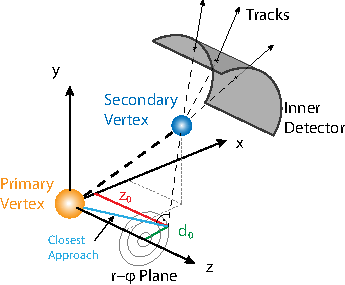
\includegraphics[width=0.49\textwidth]{SV_sketch}
    }
  \caption{(a) Example decay involving a $b$-jet (\hexbox{8AB2D3}) and jets from light flavor hadrons (\hexbox{C5C6C6}). (b) Impact parameters defined for tracks as distance of closest approach to the primary vertex for (\mbox{\color[HTML]{009245}{$d_0$}}) in the $r-\phi$-plane and for (\mbox{\color[HTML]{EC1C25}{$z_0$}}) along the z axis. (a) Adopted from \cite{Guth:2765038}.}
  \label{fig:secondary_vertex}
\end{figure} 
